On reprend ici, pour l'opération cible de dilatation, le même protocole d'expérimentation que pour l'érosion : on considère à nouveau un réseau $\mathcal{S}$MorphNetTanh qu'on munit de deux couches morphologiques, et on fixe ici l'opération cible à celle de la dilatation. On lance les différents entraînements du réseau avec l'ensemble des huit fonctions structurantes cibles considérées, avec en plus le carré binaire de taille 3x3, et ce toujours sur la banque MNIST. Tout comme pour l'érosion, on peut distinguer ici pour la dilatation deux groupes de résultats : les résultats à << succès >> de convergence, et ceux à << échec >> de convergence, tels que définis précédemment.


\newpage

\noindent Pour le carré 3x3 par exemple, à nouveau contraint par la norme $L_1$ (avec $l_c=0$) pour aider le réseau à converger correctement, on obtient l'état des deux couches morphologiques du réseau suivant, illustré figure \ref{fig:square_success_dilation} : \\

%figure
%\vspace{-1.4mm}
\begin{figure}[!htp]
  \begin{center}
    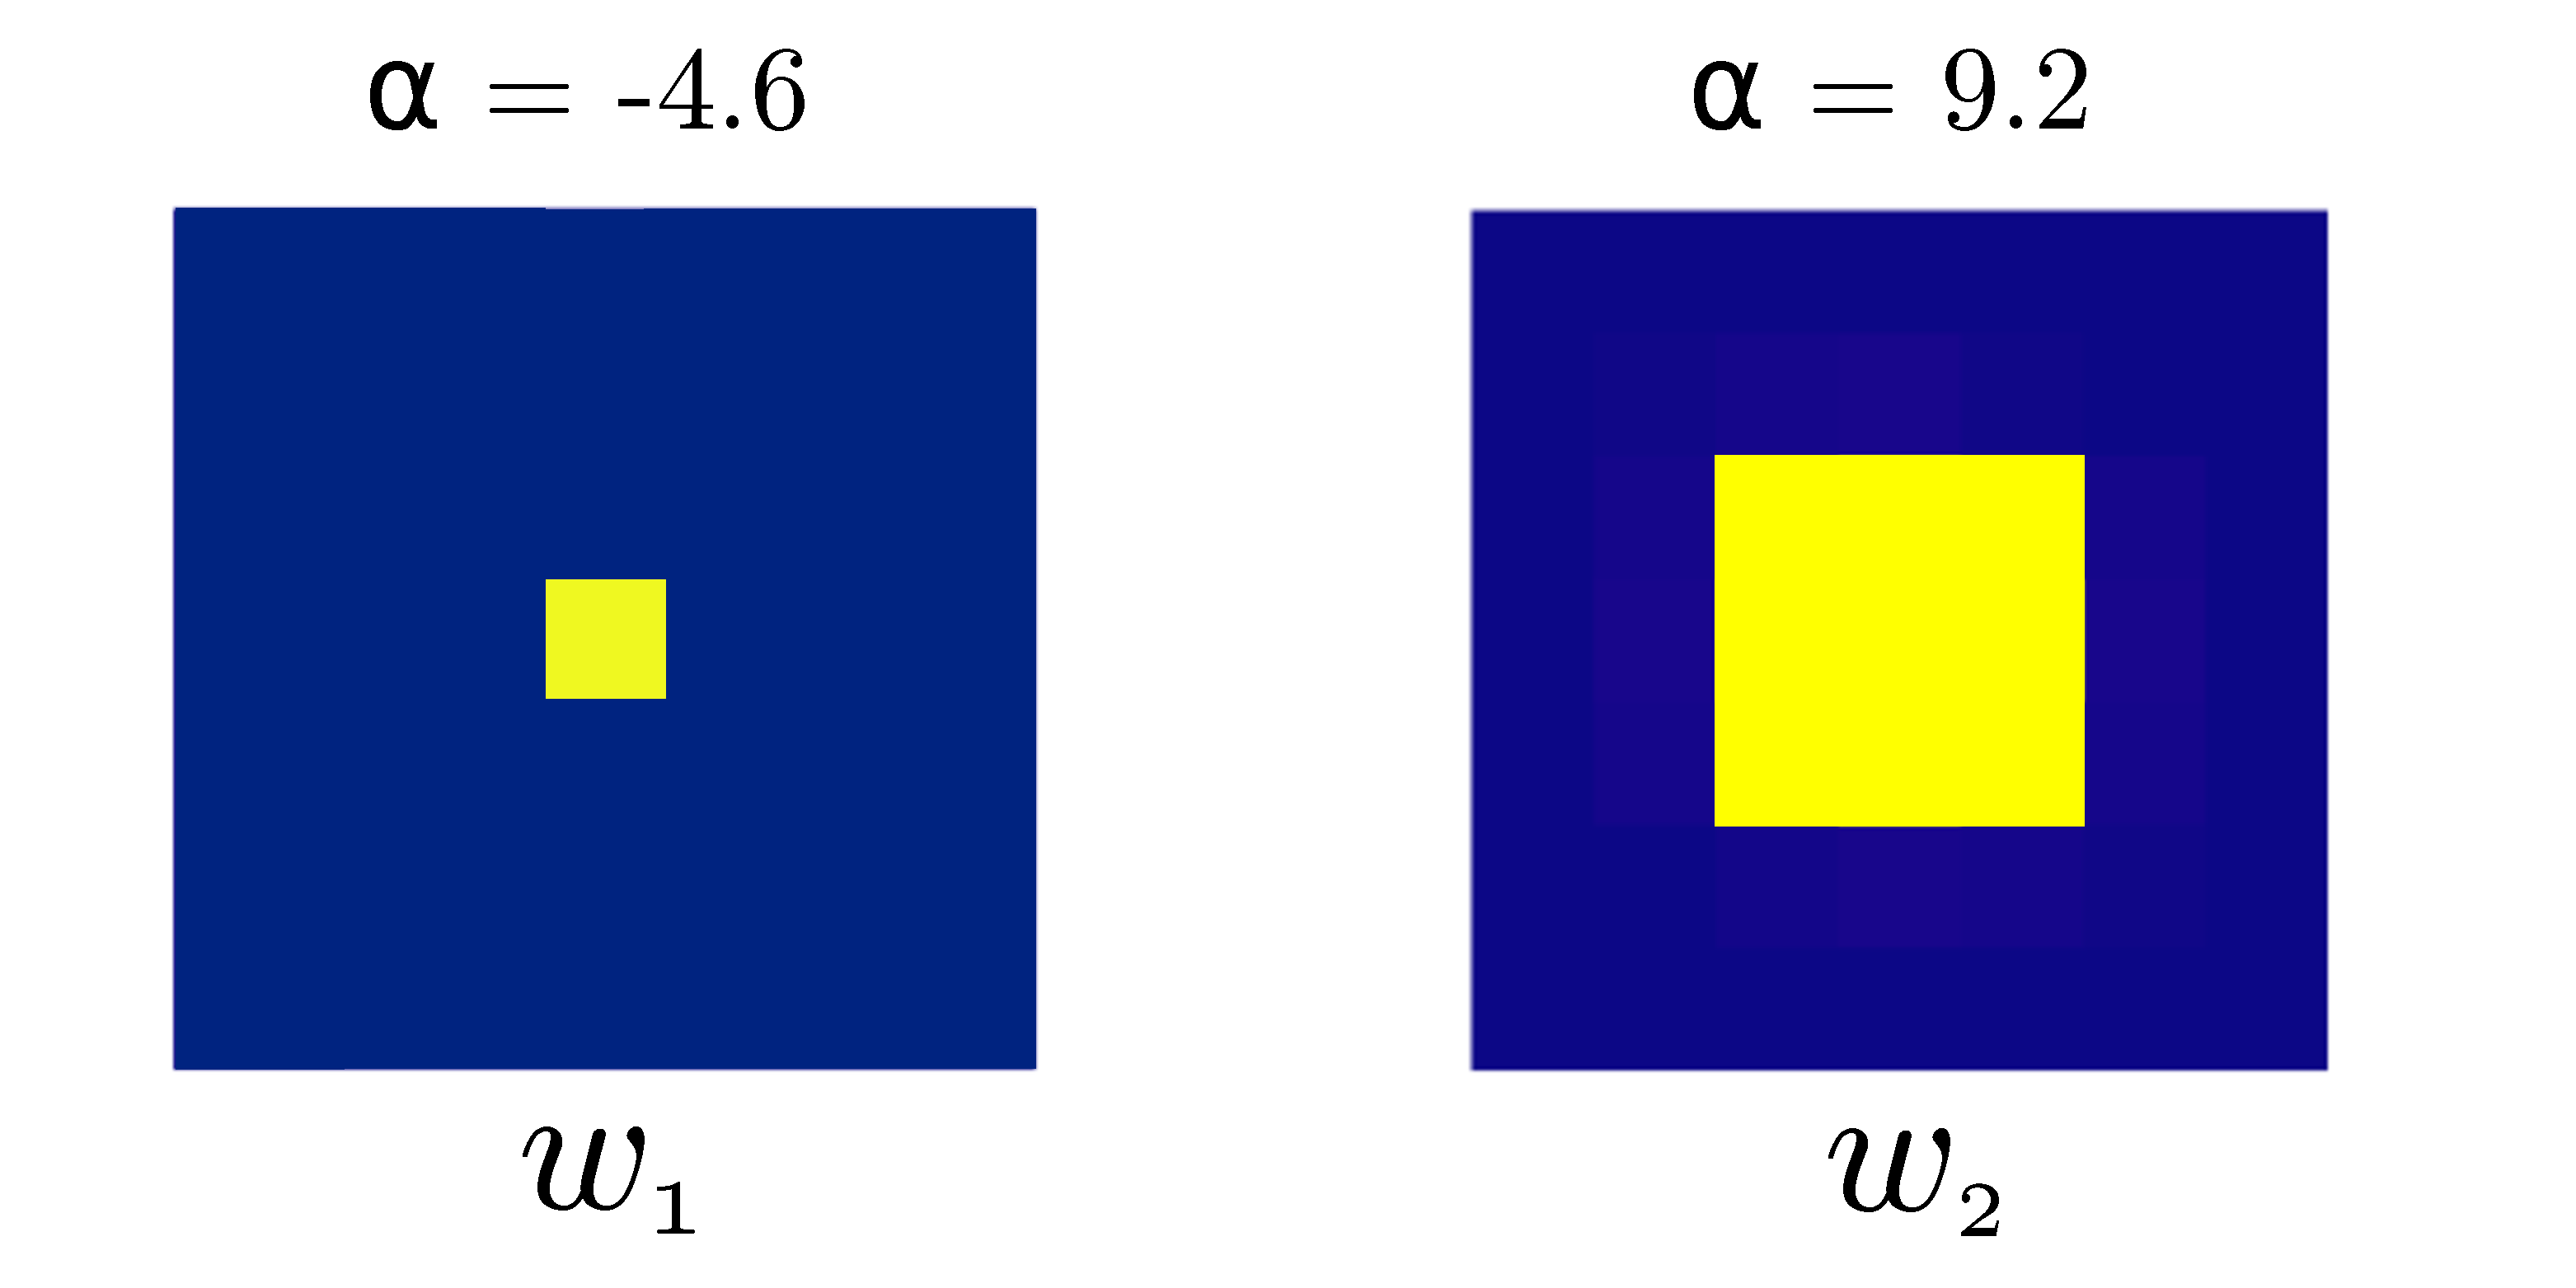
\includegraphics[width=0.36\linewidth]{parts/4-analyse_des_reseaux/deux_couches_pour_OPfondamentale/figures/square_success_dilation.pdf}
    \vspace{0.6mm}
    \caption{ \centering État final du réseau $\mathcal{S}$MorphNetTanh à deux couches morphologiques, pour la fonction structurante cible carrée 3x3 et l'opération cible de \textbf{dilatation} sur la banque MNIST, avec une contrainte des noyaux sur la norme $L_1$. Résultat : succès.}
    \label{fig:square_success_dilation}
  \end{center}
\end{figure}

\vspace{-2.0mm}
On peut à nouveau constater ici, dans le groupe des succès, l'uniformisation des solutions trouvées dans la décomposition de la fonction structurante cible par le réseau à deux couches. Sauf que, pour le cas de la dilatation, l'ordre entre structure cible et identité est inversée par rapport à celle de l'érosion : on a d'abord l'identité sur le noyau $w_1$ de la première couche, avec un $\alpha$ négatif, puis on a la forme de la structure cible sur le noyau $w_2$ de la seconde couche, avec un $\alpha$ positif. Pour l'exemple du carré 3x3, on a ainsi d'abord l'identité sur $w_1$, puis le carré 3x3 sur $w_2$ (fig. \ref{fig:square_success_dilation}). On remarque à nouveau que, d'une manière générale, l'amplitude des $\alpha$ reste faible.

\vspace{2.2mm}
